\textbf{COLUNI 2022 -- Questão 38}\par\medskip Observe o mapa abaixo, relativo aos regimes políticos da América Latina.

% COLUNI-AUTO-FIGURES-BEGIN
\begin{figure}[htbp]
\centering
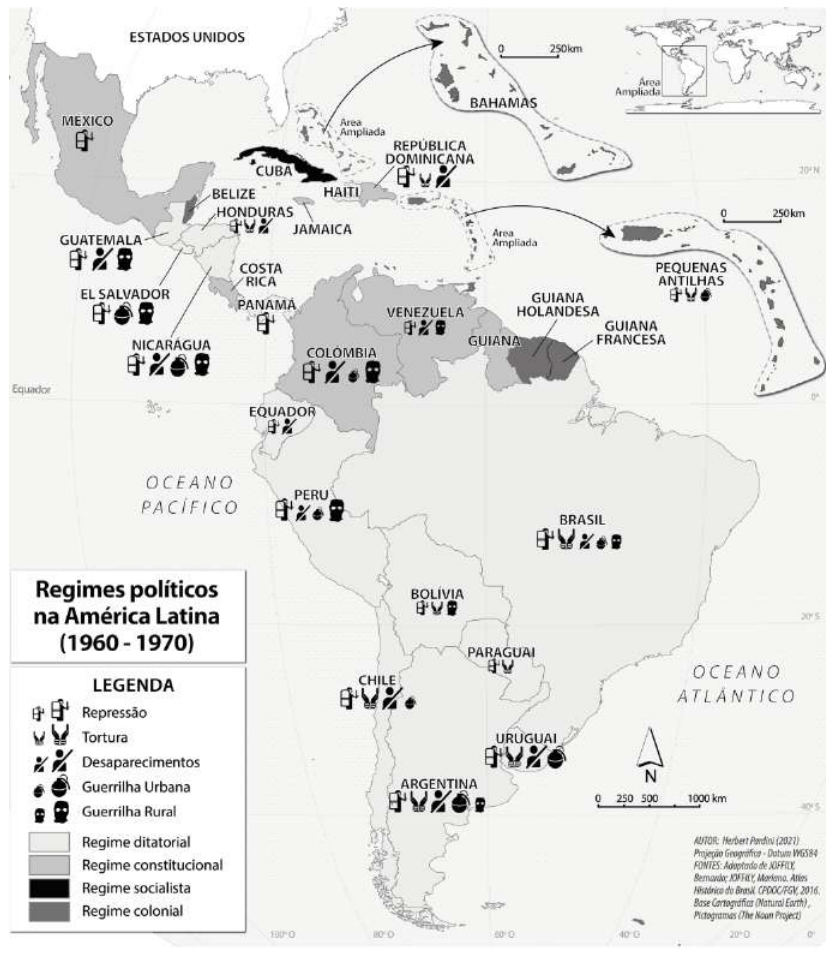
\includegraphics[width=0.95\linewidth]{static/simulados/coluni/figuras/2022/questao-38/figura-1.png}
\end{figure}
% COLUNI-AUTO-FIGURES-END

AUTOR: Herbet Pardini (2021) Projeção Geográfica - Datum WGS84. Fontes: Adaptado de JOFFILY, Bernardo; JOFFILY, Mariana. Atlas Histórico do Brasil. CPDOC/FGV, 2016. Base Cartográfica (Natural Earth), Pictogramas (The Noun Project)

\par



\par

Como se pode perceber, além do Brasil, outros países da América Latina viveram sob regime de ditadura militar. A instalação desses regimes ocorreu entre os anos 1950 e 1970, por parte de grupos capitalistas e conservadores latino-americanos que, ao apoiarem os golpes militares, tinham como finalidade impedir que o exemplo de Cuba se repetisse em outros países e barrar o avanço do comunismo.

\par

Sobre as ditaduras ocorridas na América Latina, é INCORRETO afirmar que:


\begin{enumerate}
\item os governos militares do Brasil, do Chile e da Argentina, bem como seus apoiadores civis, consideravam
      um mesmo grupo como inimigo da nação: os comunistas. Isso criou condições para o estabelecimento de
      cooperação entre os aparatos repressivos desses países.
\item a influência liberal (ou neoliberal) serviu de fundamento da política econômica no Brasil, sendo notável
      nesse país a aprovação de medidas para redução do papel do Estado, promoção de privatizações e
      abertura aos investimentos estrangeiros.
\item a resistência de diversos grupos civis latino-americanos às ditaduras militares, dentre os quais se destacam
      movimentos de mulheres, como as Mães da Praça de Maio na Argentina, permitiram o surgimento de grupos
      de luta, organização de movimentos sociais e mobilização em defesa de presos políticos.
\item a instalação do governo do general Augusto Pinochet, com ajuda dos Estados Unidos, teve como objetivo
      estabelecer uma nova ordem política, econômica e social no Chile, montando para esse fim um aparato
      repressivo que intimidou, matou e exilou seus inimigos.\end{enumerate}
